\begin{flushright} {\tiny {\color{gray} python\_codes/fieldstone\_123/text.tex}} \end{flushright}

\lstinputlisting[language=bash,basicstyle=\small]{python_codes/fieldstone_123/keywords}

\begin{center}

\fbox{\textbf{\huge \color{teal} P}}
Code at \url{https://github.com/cedrict/fieldstone/tree/master/python_codes/fieldstone_123}
\end{center}

\par\noindent\rule{\textwidth}{0.4pt}

{\sl This fieldstone was partially co-developed in collaboration with Lukas van de Wiel}. \index{contributors}{L. van de Wiel}

\par\noindent\rule{\textwidth}{0.4pt}
%%%%%%%%%%%%%%%%%%%%%%%%%%%%%%%%%%%%%%%%%%%%%%%%%%%%%%%%%%%%%%%%%%%%%%%%%%%%%%%%%%%%%%%%%%%%%%

%------------------------------
\subsubsection*{Love's problem (experiment=1)}

This problem was first published by \textcite{love29} (1929)
but we here rely on \textcite{bebe04} (2004).
The domain is a cuboid of size $L_x\times L_y \times L_z$ with $L_x=L_y=\SI{5}{\km}$
and $L_z=\SI{2.5}{\km}$. It is filled with a single elastic material characterised 
by $E=\SI{0.6e11}{\pascal}$ and $\nu=0.25$. Gravity is set to zero.
This corresponds to $\lambda= \SI{24}{\giga\pascal}$ and $\mu=\SI{24}{\giga\pascal}$.

We consider the surface displacements generated by an 
applied pressure equivalent to $\SI{100}{\meter}$ 
water depth in a rectangular area $2a\times 2b = 2\times 1~\si{\km}$. 

\begin{center}
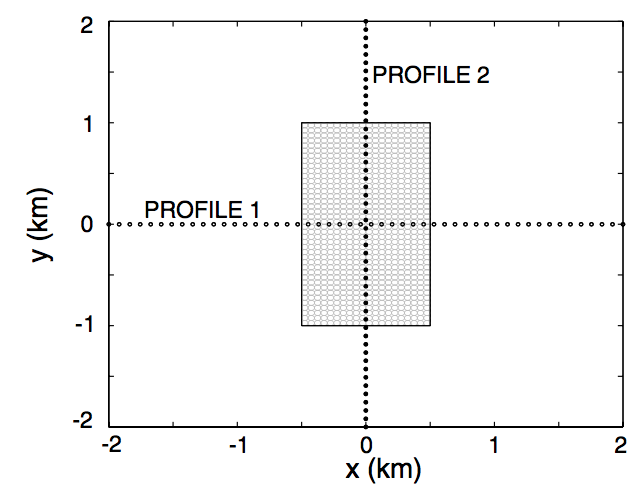
\includegraphics[width=6cm]{python_codes/fieldstone_123/images/fig1}\\
{\captionfont Top view of the problem. The gray area represents where 
pressure is applied. Note that we use a domain of different size.}
\end{center}

Because of the inherent symmetry of the problem we model only one quarter ('the top right')
of the problem. Boundary conditions are as follows: The analytical solution,
which is valid for a semi-infinite half-space, is prescribed on 
all sides and bottom while traction boundary conditions are prescribed on a 
rectangle of size $a\times b$ (the rest of the surface is left free).
This traction b.c. finds its way in the rhs. It concerns the $z$-component of
nodes 4,5,6,7, i.e. dofs 14,17,20,23. Note that it is not applied on the sides 
where the displacement is prescribed.
The analytical solution of this problem is is the {\pythonfile love.py} file.
$Q_1$ elements are used. 

\begin{center}
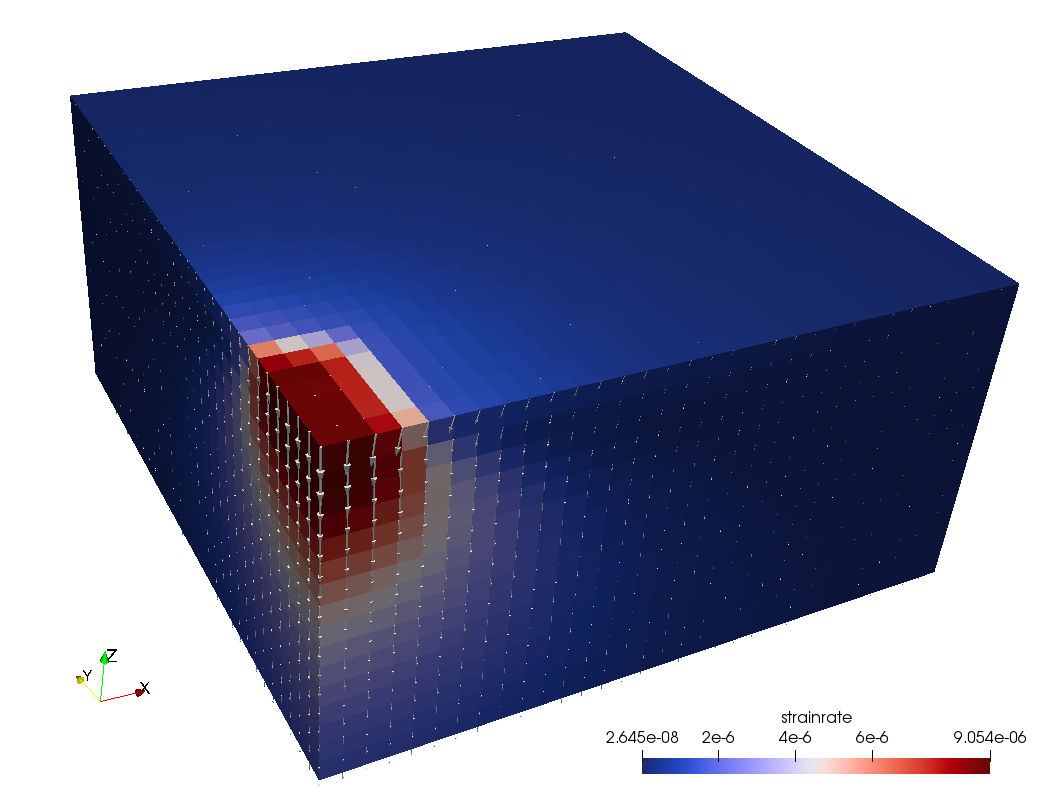
\includegraphics[width=8cm]{python_codes/fieldstone_123/results/exp1/disp} 
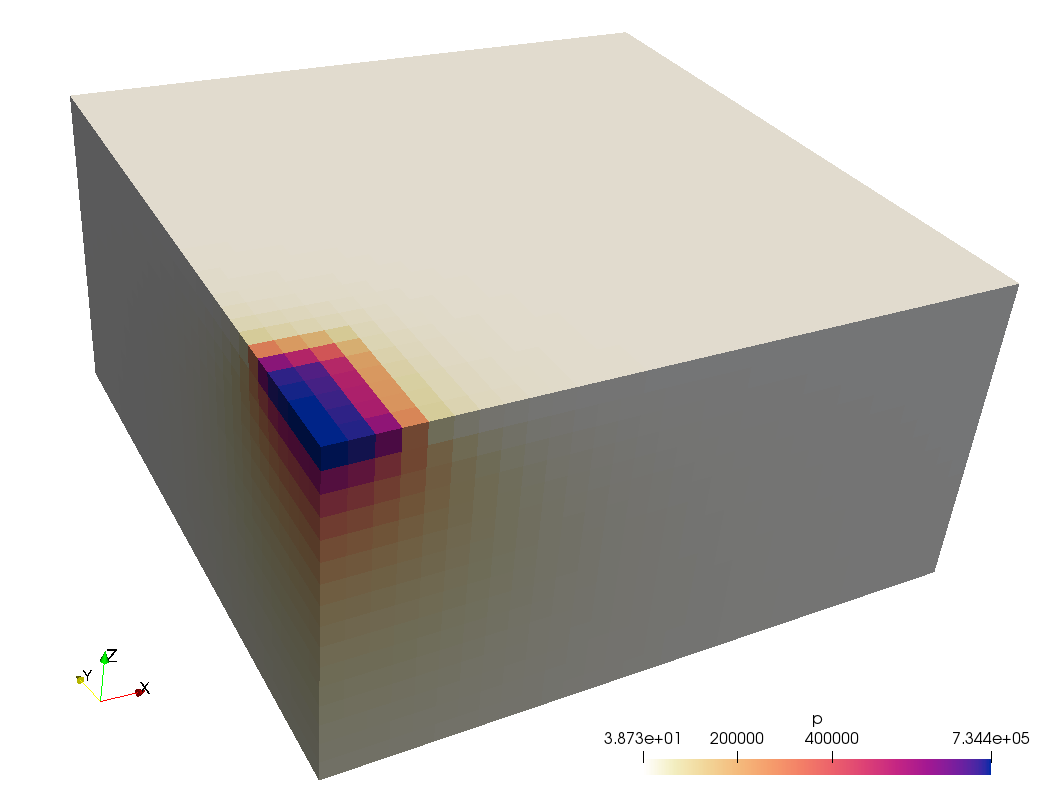
\includegraphics[width=8cm]{python_codes/fieldstone_123/results/exp1/press} \\
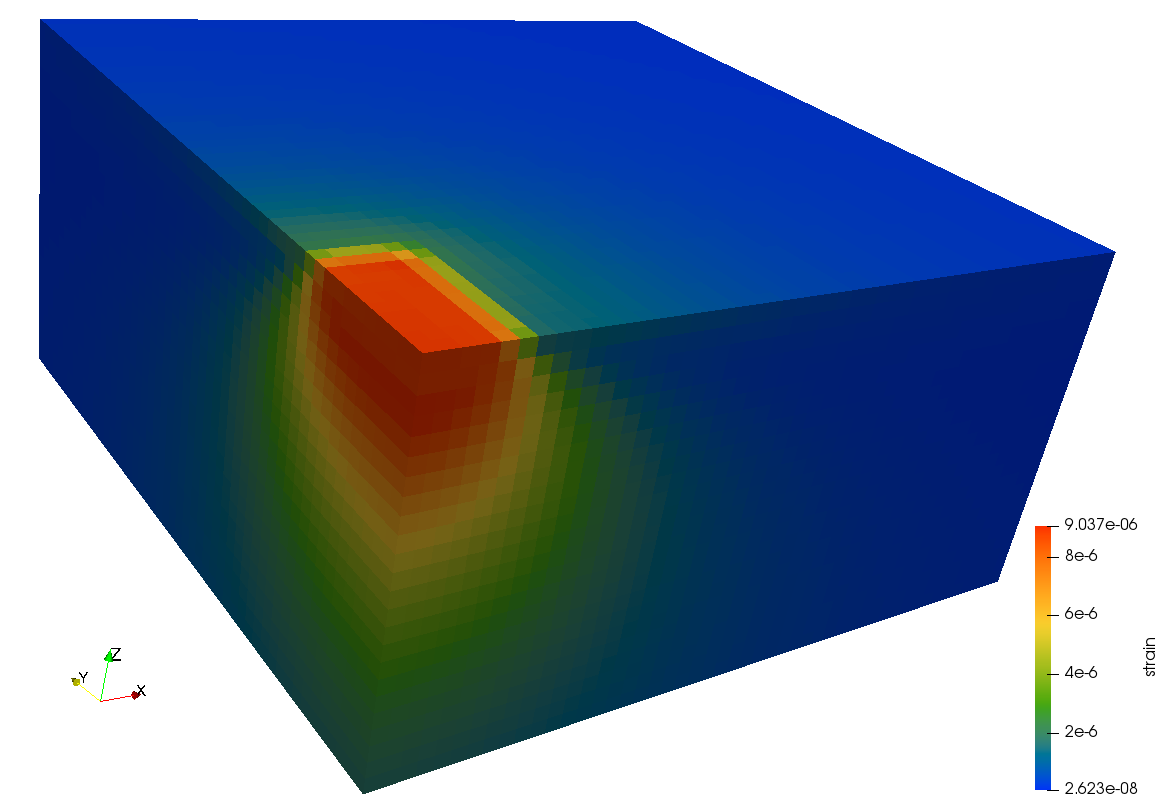
\includegraphics[width=8cm]{python_codes/fieldstone_123/results/exp1/strain} 
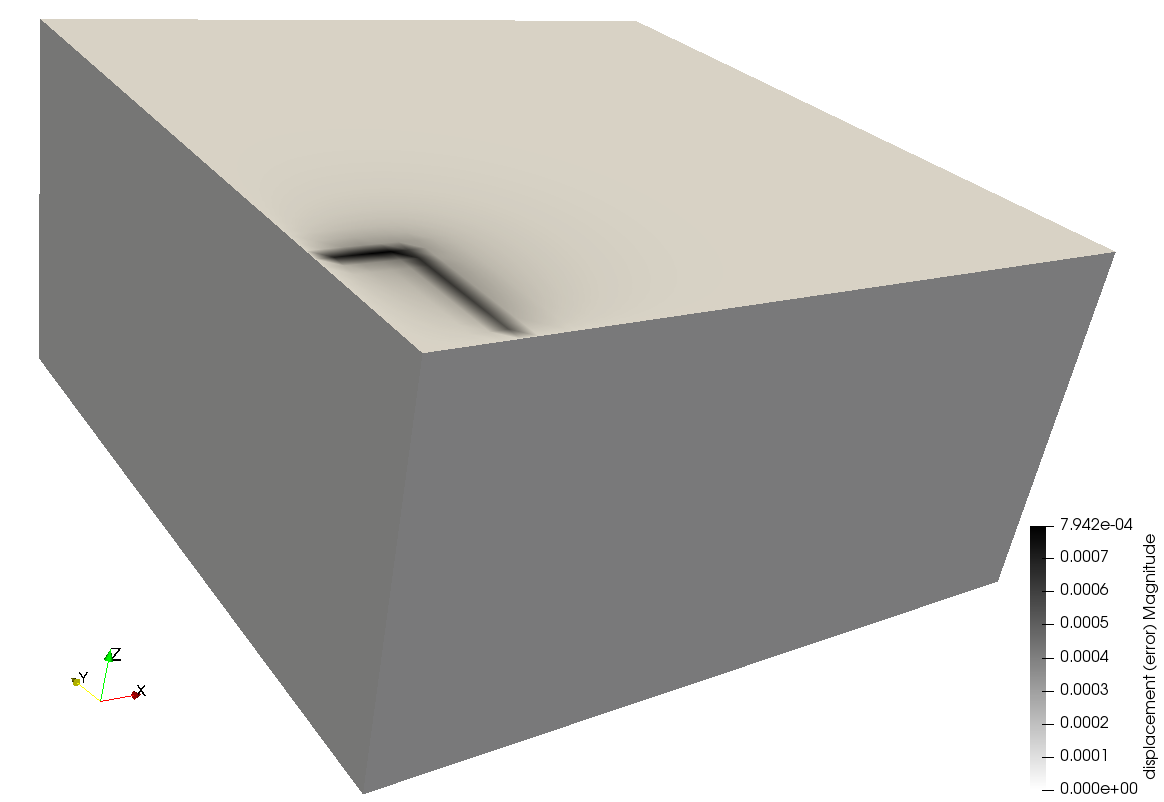
\includegraphics[width=8cm]{python_codes/fieldstone_123/results/exp1/error} \\
{\captionfont Displacement field, pressure, effective strain rate and 
displacement error on a $50\times 50\times 25$ mesh.}
\end{center} 

As in \textcite{bebe04} the displacement components are plotted on surface profiles
and are found to agree very well with the analytical solution:

\begin{center}
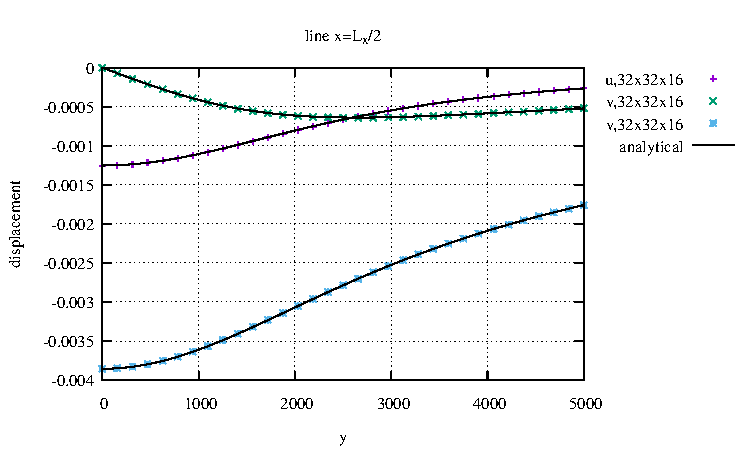
\includegraphics[width=8.2cm]{python_codes/fieldstone_123/results/exp1/xprofile.pdf} 
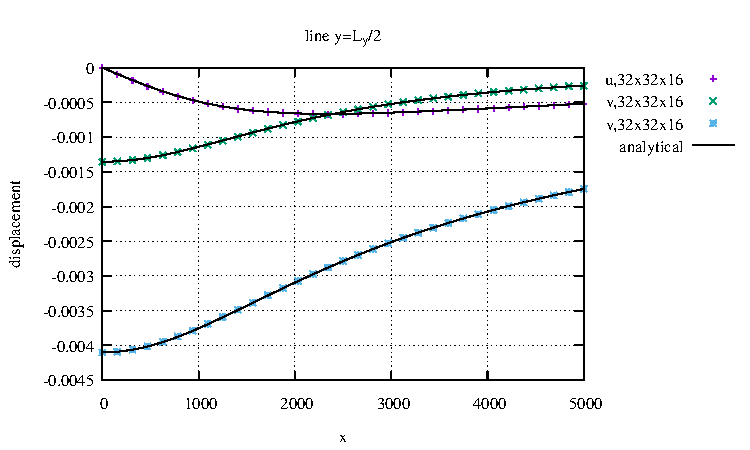
\includegraphics[width=8.2cm]{python_codes/fieldstone_123/results/exp1/yprofile.pdf} \\
{\captionfont Three components of the displacement vector $\vec{\upupsilon}$
on $x=L_x/2$ and $y=L_y/2$ lines.}
\end{center}


%----------------------------------
\subsubsection*{Boussinesq problem (experiment=2)}

We now focus on the classical Boussinesq problem (also sometimes called Boussinesq–Cerruti 
solution\footnote{\url{https://en.wikipedia.org/wiki/Linear_elasticity}}).

It consists of a point force at the origin of an infinite isotropic half-space. In the literature the 
$z$-axis is taken pointing downwards so that the force load is then $P\delta(x)\delta(y) \vec{e}_z$.
The analytical solution in Cartesian coordinates is as follows:

%r&=&\sqrt{x^2+y^2} \nn\\
\begin{eqnarray}
R&=&\sqrt{x^2+y^2+z^2} \nn\\
\upupsilon_x &=& \frac{Px}{4\pi \mu R} 
\left(\frac{z}{R^2}-\frac{1-2\nu}{R+z}\right) \nn\\
\upupsilon_y &=& \frac{Py}{4\pi \mu R} 
\left(\frac{z}{R^2}-\frac{1-2\nu}{R+z}\right) \nn\\
\upupsilon_z &=& \frac{P}{4\pi \mu R} 
\left(2(1-\nu)+\frac{z^2}{R^2}\right) \nn\\
\sigma_{xx} &=& -\frac{P}{2\pi R^2}
\left[\frac{3x^2z}{R^3}-(1-2\nu)\left(\frac{z}{R}-\frac{R}{R+z} + \frac{x^2 (2R+z)}{R(R+z)^2}\right)
\right]\nn\\
\sigma_{yy} &=& -\frac{P}{2\pi R^2}
\left[\frac{3y^2z}{R^3}-(1-2\nu)\left(\frac{z}{R}-\frac{R}{R+z} + \frac{y^2 (2R+z)}{R(R+z)^2}\right)
\right]\nn\\
\sigma_{zz} &=& -\frac{3Pz^3}{2\pi R^5} \nn\\
\sigma_{xy} &=& -\frac{P}{2\pi R^2} 
\left(
\frac{3xyz}{R^3} - (1-2\nu) \frac{xy(2R+z)}{R(R+z)^2}
\right) \nn\\
\sigma_{xz} &=& -\frac{3Pxz^2}{2\pi R^5} \nn\\
\sigma_{yz} &=& -\frac{3Pyz^2}{2\pi R^5} \nn
\end{eqnarray}

The domain and material parameters are identical to those of the previous benchmark. The load is 
set to $\SI{100}{\giga\pascal}$ and set at $x=L_x/2,y=L_y/2$.
The solution is unfortunately singular where the load is applied, and this translates numerically in displacements
that become larger and larger just below it. However, a few elements away from the singularity the 
analytical solution is recovered (Note that the analytical solution is set to zero at the point load - 
see {\pythonfile boussinesq.py}):

\begin{center}
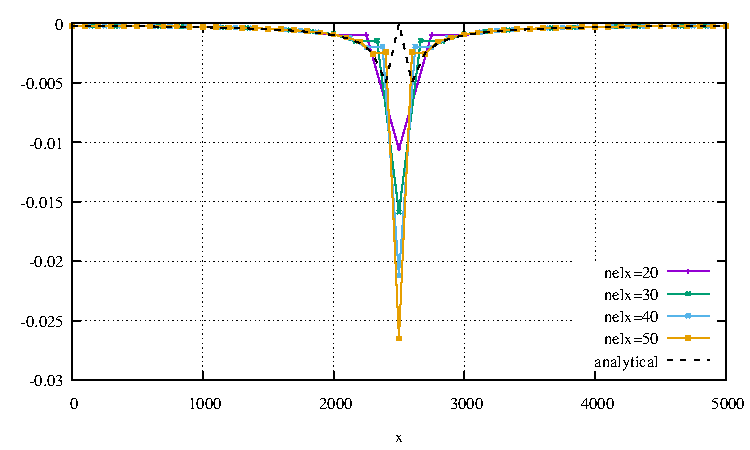
\includegraphics[width=5.7cm]{python_codes/fieldstone_123/results/exp2/xprofile_uz.pdf}
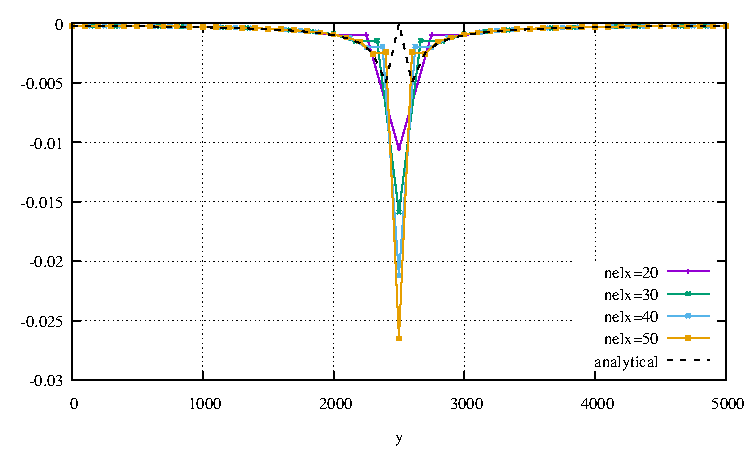
\includegraphics[width=5.7cm]{python_codes/fieldstone_123/results/exp2/yprofile_uz.pdf}
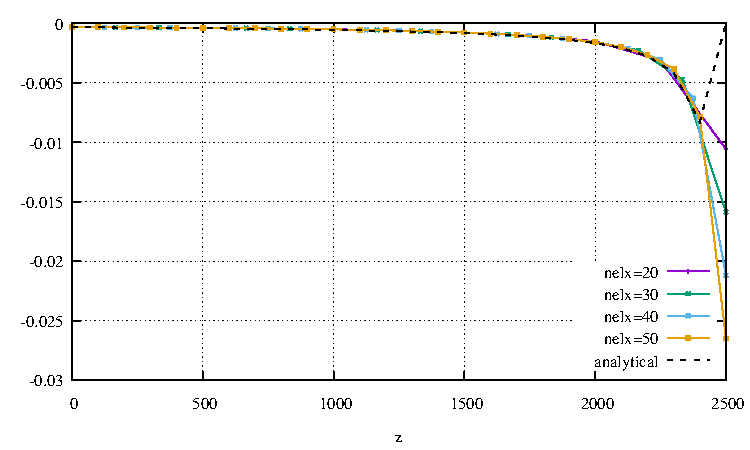
\includegraphics[width=5.7cm]{python_codes/fieldstone_123/results/exp2/zprofile_uz.pdf}\\
{\captionfont Vertical component of the displacement as measured on horizontal and 
vertical lines passing through the point load.}
\end{center}



\begin{center}
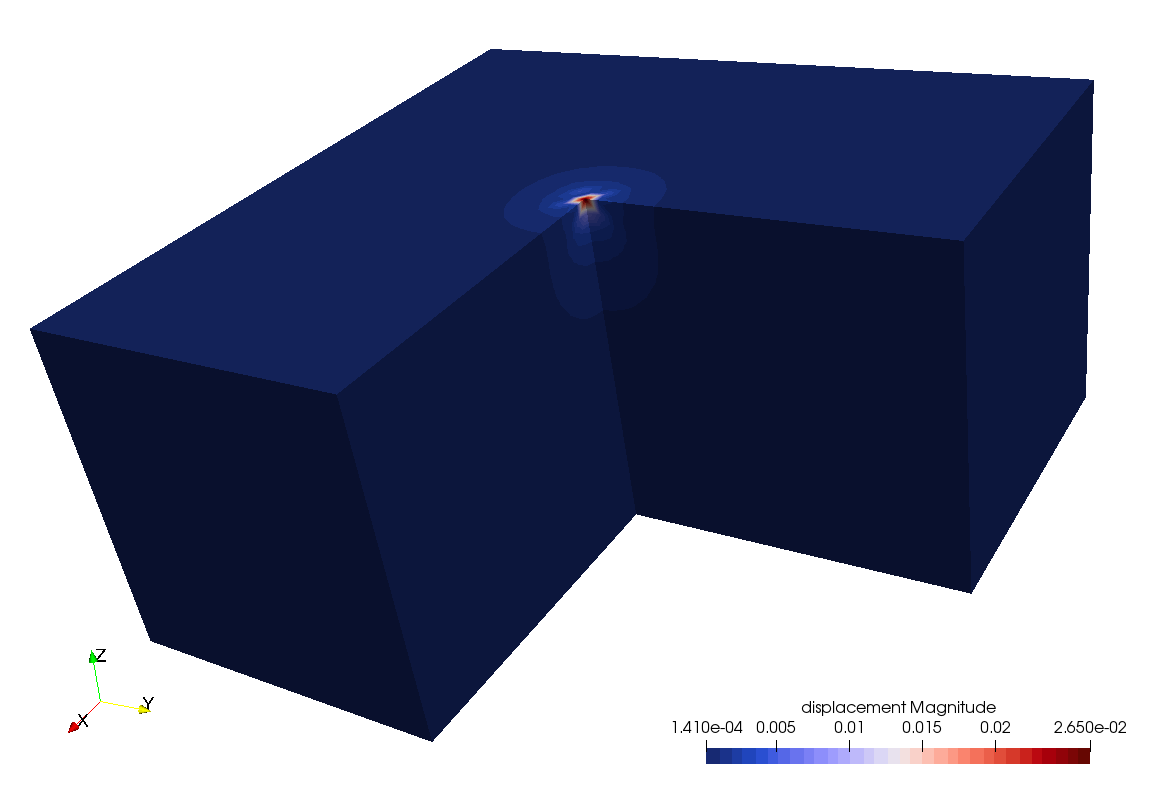
\includegraphics[width=5.27cm]{python_codes/fieldstone_123/results/exp2/50/disp} 
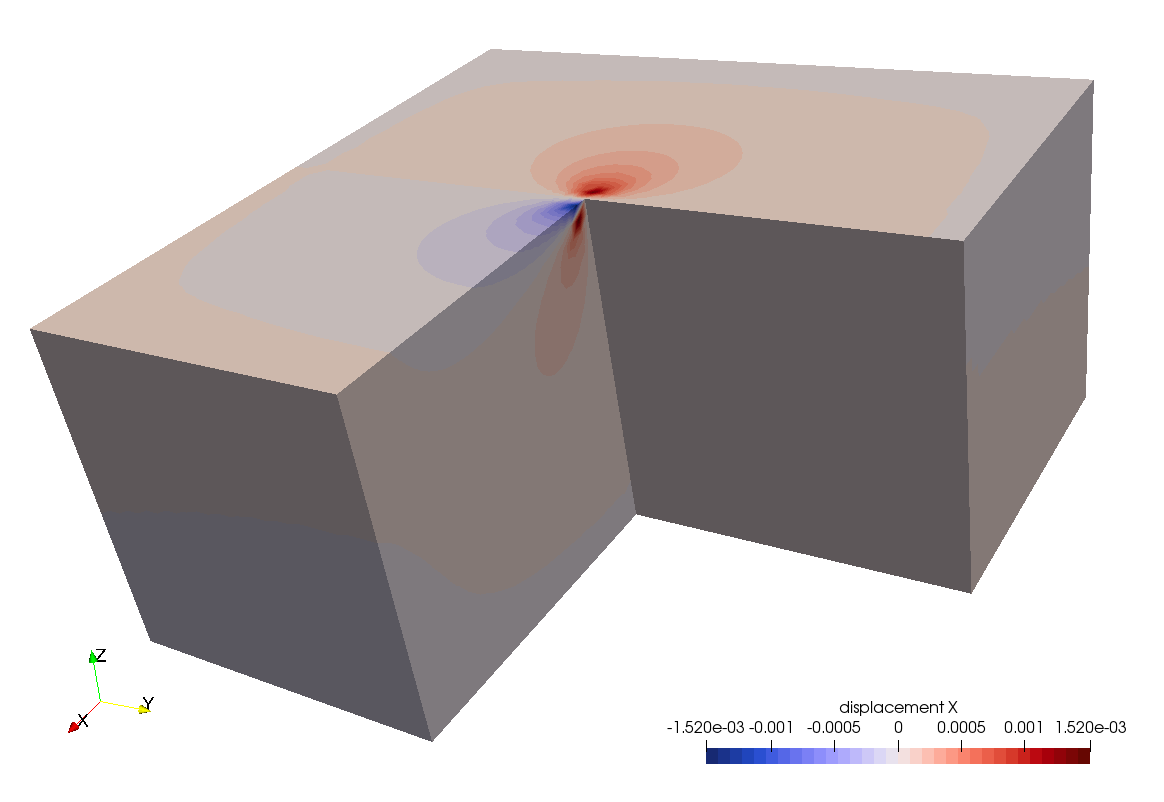
\includegraphics[width=5.27cm]{python_codes/fieldstone_123/results/exp2/50/dispx} 
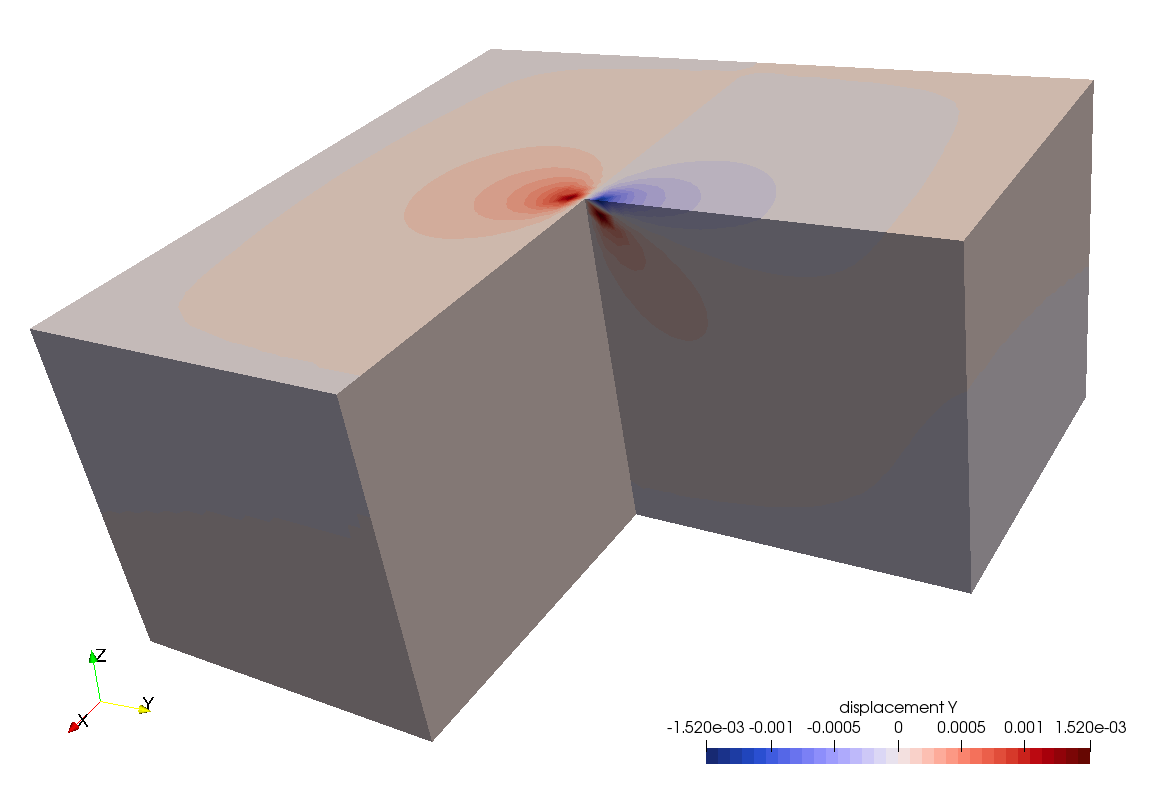
\includegraphics[width=5.27cm]{python_codes/fieldstone_123/results/exp2/50/dispy} \\
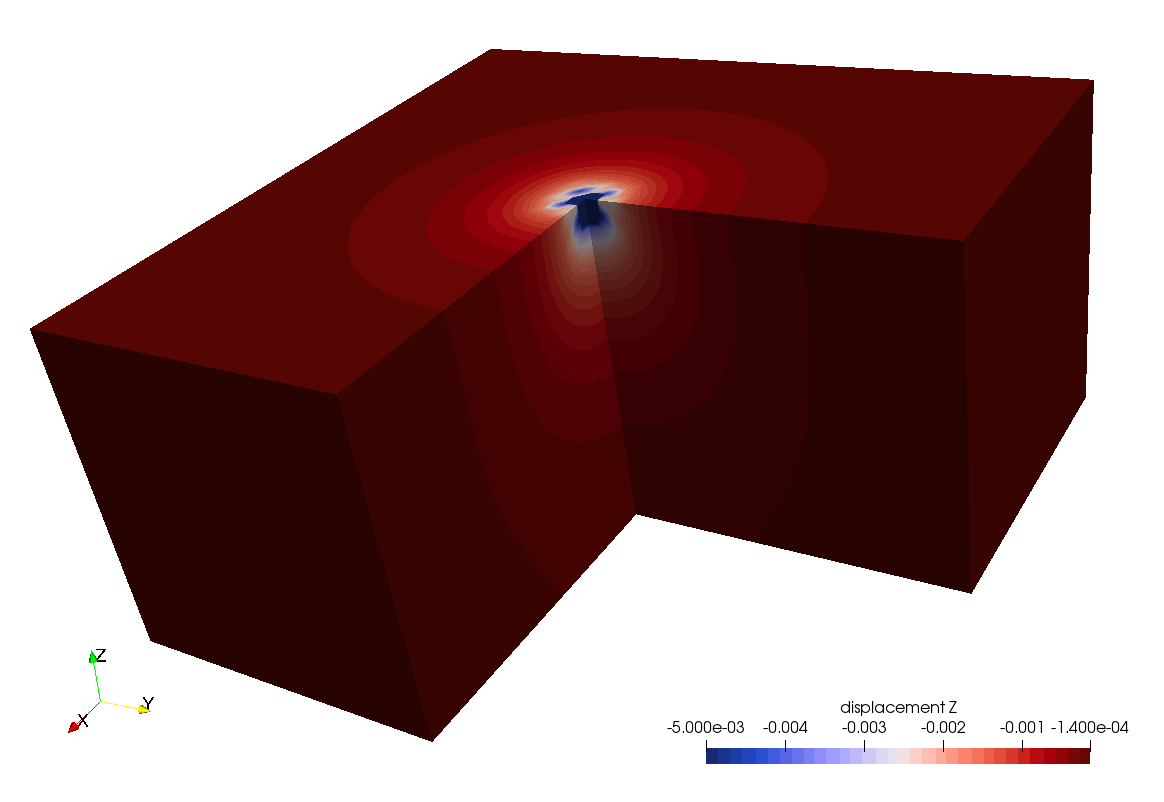
\includegraphics[width=5.27cm]{python_codes/fieldstone_123/results/exp2/50/dispz} 
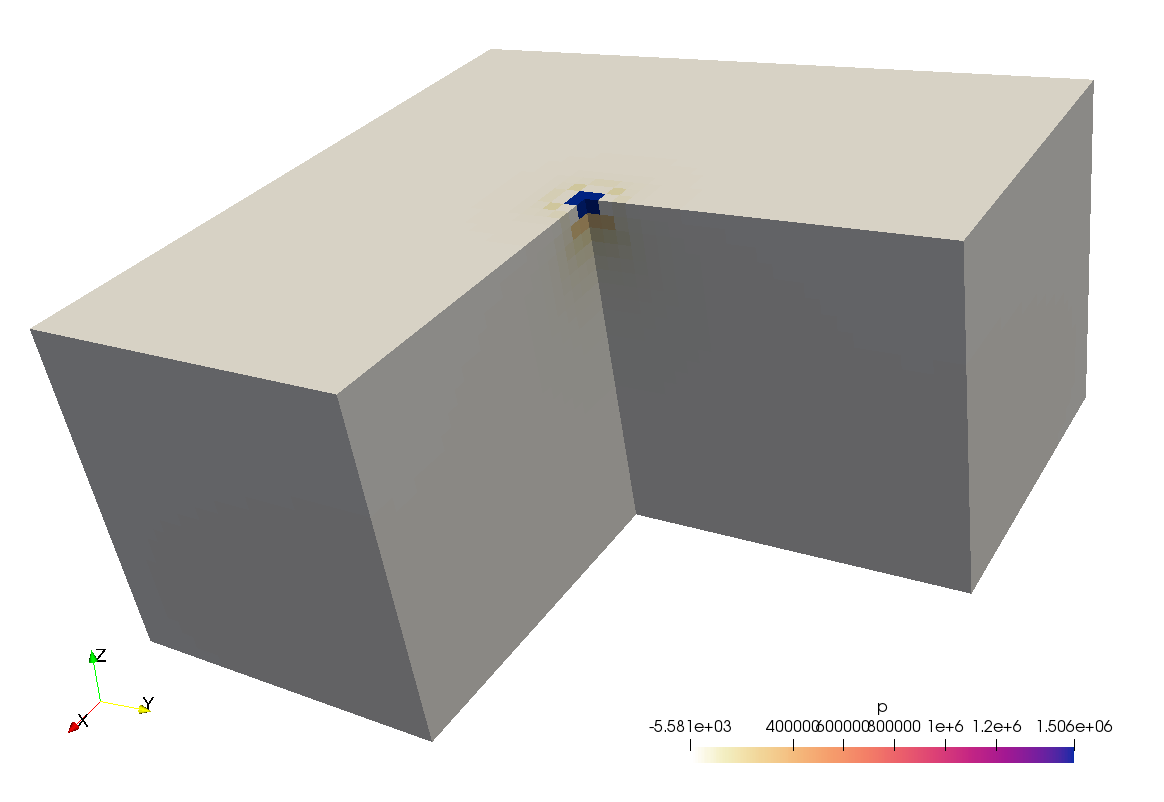
\includegraphics[width=5.27cm]{python_codes/fieldstone_123/results/exp2/50/press} 
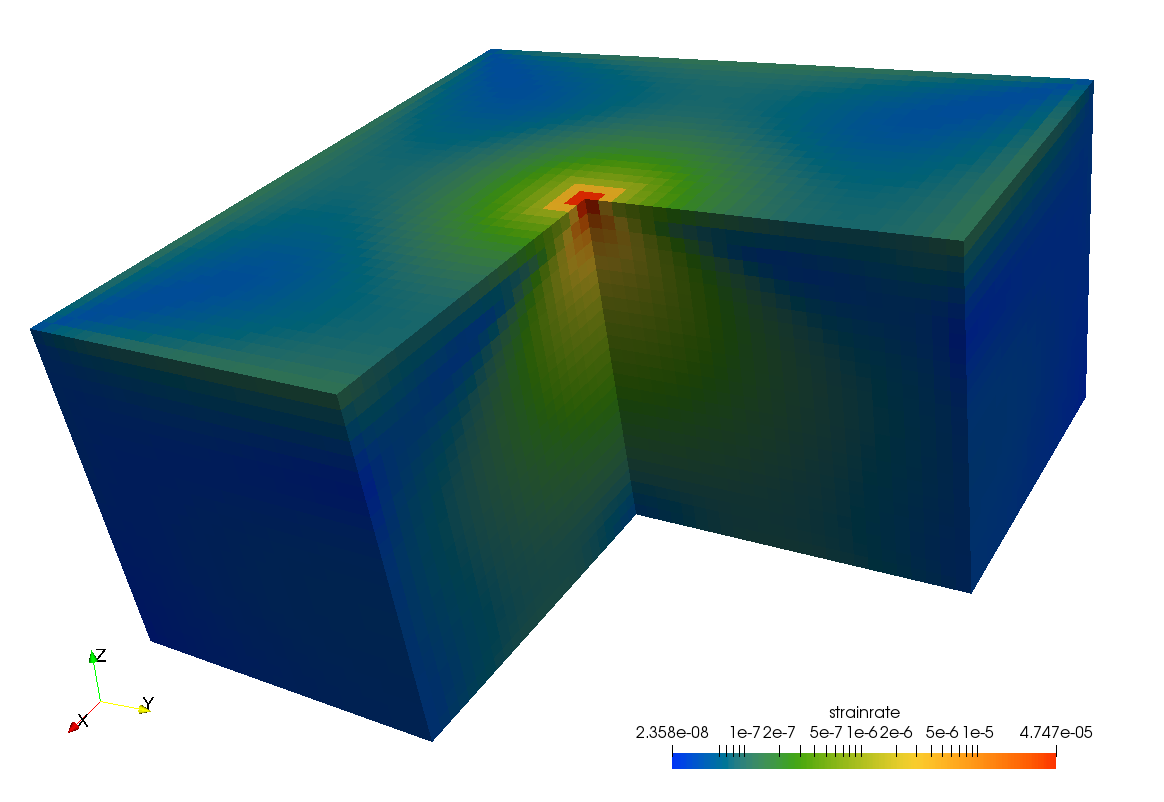
\includegraphics[width=5.27cm]{python_codes/fieldstone_123/results/exp2/50/strain}\\ 
{\captionfont Various fields as obtained on a $50\times 50 \times25$ mesh
which seems to be about the maximum resolution. It takes over 10min to run and uses about 16Gb of RAM.}
\end{center}




